\chapter{Multi-Modal Interaction-Aware Trajectory Optimization}
\label{text:approach}

To the best of the author's knowledge, exploiting the gradient of a deep neural network for trajectory optimization has not been done before, likely due to the tight runtime requirements of an online optimization as well as the lack of guarantees and insights that can be retrieved from such an approach without further ado. Several approaches have dealt with data-driven prediction models outputs before. Accessing the model's internal structure enables computing gradients that are more informed about the actual interactions happening in a multi-agent scene beyond the trajectory predictions. However, computing a gradient by backward passing through the whole network is widely associated with sizeable computational effort. While this may be true in general, trajectory optimization networks and input data are comparably small enough to perform these computations efficiently. 

\begin{figure}[!ht]
\begin{center}
\begin{tikzpicture}

	\pie[radius=2.2, explode={0, 0, 0.2, 0}] {14.6/data-processing , 17.7/forward-pass , 19.0/backward-pass , 40.2/loss-evaluation, 1.5/others,  7.0/evaluation} 
	
\end{tikzpicture}
\end{center}
\caption{Runtime evaluation of training the Trajectron model \cite{Salzmann2020} on pre-processed data of the ETH Hotel 2 pedestrian dataset \cite{Pellegrini2009}}
\label{img:training_runtime}
\end{figure}

Figure \ref{img:training_runtime} gives an inside into the runtime distribution of the Trajectron model, during training. Here, merely roughly one-fifth of the overall runtime is spent performing the backward pass, while most time is spent evaluating the loss function. In particular, forward- and backward-pass do not differ much regarding their overall runtime. While this is only one out of many examples, it illustrates the capability of performing a backward pass online.  
\newline\newline
In this chapter, an overview of the approach is provided. In Section \ref{text:approach/formulation}, the problem of socially aware motion planning is formulated formally, including the assumptions made within this project. 
\newline
Section \ref{text:approach/overview} presents an overview of the full trajectory optimization pipeline. It is shown how the algorithm is built to allow us to deal with general graph-like pedestrian behavior prediction models, with multimodal, probabilistic outputs. Furthermore, the advantages of formulating socially aware motion planning as an optimization problem while utilizing a graph-based prediction model, e.g., deep learning-based models such as the Trajectron \cite{Ivanovic2018}, over purely learned \cite{Chen2017} or purely optimization-based \cite{Berg2011} algorithms are illustrated. Finally, it is explained how the usage of a general-purpose, computation-graph-based framework such as PyTorch \cite{pytorch} or TensorFlow \cite{tensorflow} can be harnessed for a highly modular, efficient, and versatile implementation.
\newline
The optimization problem's exact formulation is further explained in Section \ref{text:approach/objective} and \ref{text:approach/constraint}. Both the goal-driven and the interaction-driven parts are illustrated, beginning with the objective function and continuing with a derivation of their gradients. Furthermore, several designs of the specific objective function are discussed. The subsequent section addresses the design of the constraints used. Likewise, several constraint function designs are compared. 
\newline
To use the system in real-world applications, it must comply with several requirements. While the optimization design has tackled some of these, e.g., the feasibility of the robot's control limitations or safety regarding robot-human interaction, the system underlies runtime limits. Several runtime improvements have been implemented to achieve this goal, which are described in Section \ref{text:approach/runtime}.


\section{Problem Formulation}
\label{text:approach/formulation}
In this work, we are interested in finding the optimal trajectory for a robot navigating among pedestrians on the two-dimensional plane. Let $\x_t = (x_t, y_t) \in \mathbb{R}^2$ and $\dx_t = (\dot{x}_t, \dot{y}_t) \in \mathbb{R}^2 $ be the position and velocity of the robot, also referred to as $ego$, at time $t$ and $(\x, \dx)_{0:N}$, a trajectory over multiple position-velocity-pairs $((\x, \dx)_0, (\x, \dx)_1, (\x, \dx)_2, \hdots, (\x, \dx)_N)$. Within this work, the robot is assumed to have double integrator dynamics. With control input $\u_t = (u_{x, t}, u_{y, t}) \in \mathbb{R}^2$, we have: 

\begin{equation}
\ddx_t = \u_t
\label{eq:robot_dynamics}
\end{equation}

For further simplification, the robot's dynamics are assumed to be deterministic. 
The pedestrians (also referred to as $ados$) follow single integrator dynamics. As pointed out in \cite{Ivanovic2018}, this is a natural choice "as a person's movements are all position-changing, e.g., walking increases position along a direction, running does so faster." Other standard models for pedestrian dynamics such as Social Forces \cite{Helbing1995}, however, regard the pedestrian to be a double integrator, not a single integrator, and describe the forces acting on it introduced by other pedestrians and obstacles. Having a reasonable fast reaction time and a large maximal acceleration in comparison to the robot, both of these descriptions converge so that the single integrator model is the right choice nonetheless. \footnote{As discussed in Chapter \ref{text:experiments} the modular implementation allows us to use different pedestrian dynamics. When testing against other prediction environments non-single integrator dynamics are used, but most analysis described in this report relates to the single integrator model.}

\begin{align}
\dxped[k]_t = \uped[k]_t
\label{eq:pedestrian_dynamics}
\end{align}

Each pedestrian's future trajectory is predicted as a probabilistic and multimodal using some model $\distmodel[]$. Thereby, let $\xped[k]_t \sim \dist[k]_t$ be the distribution of the pedestrian $k$s velocity at time $t$, with mean $\muped[k]_t$, variance $\sigmaped[k]_t$, and mode-weights vector $\piped[k]_t$. The prediction is based on the past states of the robot $\x_{0:t}$ and of every pedestrian in the scene $\xped[j]_{0:t}$, including pedestrian $k$. Moreover, the function $\distmodel[]$ is generally not shared across all pedestrians but individually for each one.

\begin{align}
\xped[k]_t &\sim \distmodel[k]_t(\muped[k]_t, \sigmaped[k]_t, \piped[k]_t) \\
\dist[k]_t &= \distmodel[k] (\x_{0:t}, \xped[0]_{0:t}, \hdots, \xped[K]_{0:t})
\end{align}

Like the robot, the pedestrians are modeled as single point masses, both underlying speed bounds defined by the $L_2$ norm of their velocities. Furthermore, both the robot and the pedestrians underly constraints for their minimal and maximal control effort. Thus, the sets of feasible control inputs $
\uset$ and $\upedset$ respectively, are defined using the $L_1$-norm and the $L_2$-norm respectively:

\begin{align}
\uset &= \{\u | \u \in \mathbb{R}^2, ||\u||_1 \leq u_{max}\} \\
\upedset &= \{\uped[] | \uped[] \in \mathbb{R}^2, ||\uped[]||_2 \leq \tilde{u}_{max}\} 
\label{eq:controls_bounds}
\end{align}
 
All actions are assumed to take place in a free-space, two-dimensional environment. 
\newline
Within project \project, we want to find a robot trajectory $\x_{0:T}$ over some discrete-time horizon $N$ that makes trade-offs between minimizing the travel time from its current state to some goal state in $\xset_f = \{\boldsymbol{g} | \boldsymbol{g} \in \xset \}$ on the one side and the interference with the pedestrians in the scene, concerning its dynamic as well as safety boundaries, on the other side. For further simplification, perfect knowledge about the current and all past states of surrounding agents $\xped[k]_{0:t} \forall k \in [0, K]$ is assumed.
\newline\newline
For brevity of notation, in the following, the temporal index $t$ and the pedestrian index $k$ will be omitted when not necessary.


\section{System Overview}
\label{text:approach/overview}
As shown in Figure \ref{img:information_flow} the problem can be divided into several subproblems, which also can be seen as modules of a trajectory optimization problem and therefore can be formulated independently from each other. 

\begin{figure}[!ht]
\begin{center}

\includegraphics[width=\imgwidth]{images/placeholder.png}
\caption{Information-Flow-Diagram}
\label{img:information_flow}
\end{center}
\end{figure}

Formally, the solution to this problem can be represented as the following optimization problem (compare Problem \ref{eq:formulation}), which is executed in an MPC-manner. \\

\begin{problem}{\textrm{General optimization problem}}
\begin{equation}
\min_{\u_{0:T-1}} \quad w_{goal} J_{goal} + w_{int} \sum_{k=0}^K J_{int}^k
\end{equation}
\begin{align}
\textrm{s.t. } \quad & \x_{t+1} = \f(\x_t, \u_t) & \forall t \in [0, T - 1] \\
& \xped[k] = \distmodel[k](\x_{0:t}, \xped[i]_{0:t}) & \forall k \in [0, K], \forall t \in [0, T]\\
& g_{safety}(\x_{0:T}, \xped[k]_{0:T}) \leq 0 & \forall k \in [0, K] \\
& \x_t \in \xset & \forall t \in [0, T]\\
& \u_t \in \uset & \forall t \in [0, T]\\
& \x_0 \in \xset_0
\end{align} 
\label{eq:formulation}
\end{problem}

. Due to the linear and cheap to compute dynamics, the availability of a simulation engine tightly bound to the optimization and since the constraints acting on both the path $\x_{0:T}$ itself and the controls $\u_{0:T}$ are comparably "simple", as illustrated in Section \ref{text:approach/constraint}, shooting is used within this project. Therefore the trajectory is split up into several segments, one for each discrete discretization time step, which makes solving problem \ref{eq:formulation} easier to be solved and more robust (multiple shooting) \cite{Betts1998}. In this work the initial time $t_0 = 0$ and the final time $t_f = T \cdot \Delta t$ is used for simple notation, although not required in general \cite{Wachter2006}. 
\newline
The objective function is a weighted sum of a goad-driven $J_{goal}(\cdot)$ and some interaction-driven term $J_{int}(\cdot)$, which are further explained in Section \ref{text:approach/objective}. The constraints are a combination of dynamics constraints, safety constraints as well as initial and final state restrictions, which are discussed in Section \ref{text:approach/constraint}. Note that the terminal state $\x_T$ of the planned trajectory is not constrained to be in the terminal set $\xset_f$. As stated in chapter \ref{text:introduction} within this project the safety and un-disturbed gait of pedestrians is considered to be more important than reaching the goal state time-optimally. While the goal-driven objective $J_{goal}(\cdot)$ introduces an incentive to approach the goal state, constraining the terminal state to be in the terminal set would informally speaking, remove the possibility of detouring to not interfere a pedestrians movement. 
\newline
Over Problem \ref{eq:formulation} has $2*T$ optimization variables, $(2*T + 1) + 2*T + K = 3*T + K + 1$ constraints, all of them being inequality constraints, causing $T * (T+1) + 2*T + K$ non-zero Jacobian elements.

\subsubsection{Nonlinear optimization Solver} 
Since no further assumptions about the pedestrian trajectory prediction model $\distmodel[]$ have been made, the optimization is non-linear and especially non-convex in general. As shown in \cite{Gould2003}\cite{Parkinson2018}\cite{Freund2004} there are a bunch of algorithms to deal with general non-linear optimization problems, such as line-search, trust-region, interior-point, generalized-reduced-gradient or sequential-quadratic-programming methods as well as combinations of these such as LOQO. However, not all of them apply to constrained problems such as Problem \ref{eq:formulation}. For constrained optimization problems \ac{SQP} and \ac{IPM} are the most popular ones, both having their advantages and drawbacks. While \ac{SQP} usually require fewer solver iterations and thus fewer function calls, they scale poorly with the number of constraints and do not guarantee that intermediate results are feasible \cite{Dehdari2013}\cite{Parkinson2018}. Although this can be an advantage in the case of computationally expensive constraints, it also leads to an infeasible solution when the algorithm is stopped for convergence. Additionally, compared to \ac{IPM} the computational time required by the solver itself is usually larger (e.g. as demonstrated in \cite{Dehdari2013}).
\newline
In project \project safety is induced by constraint, thus obtaining a feasible solution is crucial, also if the algorithm might be aborted before convergence due to runtime constraints. For this reason, an interior-point method has been used within the project. The idea of interior point optimization methods is to create constraint barriers that increasingly push the solution from an infeasible state to the feasible region, without pushing it too much away from the feasible border (since often the optimal solution is close to the feasible border), using a loss function combining the objective and constraint “loss” by introducing Lagrangian parameters. IPOPT especially has very good performance in recovering from some infeasible state in a “smart” manner.  Therefore it is quite robust, but hard to warm-start. 
\newline
The interior-point method \ac{IPOPT}\footnote{\ac{IPOPT} is only available for C++, the cython-based wrapper cyipopt is used.} \cite{Wachter2006} has shown to be applicable in many robotics applications, and has shown to be valuable even in case of very tough runtime constraints such as solving the feedforward commands in high-performance automated driving at 50 Hz in \cite{Spielberge2019} or motion planning for legged robotics \cite{Winkler2018}. Therefore it has been used in this project as well\footnote{From today's point of view it turned out, after tweaking the performance of the optimization core as best as possible, it turns out that the number of objective function calls is the bottleneck of the algorithm. Therefore comparing the capacity of the interior-point solver such as \ac{IPOPT} with \ac{SQP} solvers such as \ac{GuSTO} remains for future work.}.

% The NLP solver implements the following primal-dual methods for finding a local minimum: 1) interior point trust-region line-search algorithm 2)active-set trust-region line-search algorithm
%Both methods can solve small-, medium-, and large-scale optimization problems efficiently and robustly. These methods use exact first and second derivatives to calculate search directions. The memory requirements of both algorithms are reduced dramatically because only nonzero elements of matrices are stored. Convergence of both algorithms is achieved by using a trust-region line-search framework that guides the iterations towards the optimal solution. If a trust-region subproblem fails to provide a suitable step of improvement, a line-search is then used to fine tune the trust-region radius and ensure sufficient decrease in objective function and constraint violations.
%The interior point technique implements a primal-dual interior point algorithm in which barrier functions are used to ensure that the algorithm remains feasible with respect to the bound constraints. Interior point methods are extremely useful when the optimization problem contains many inequality constraints and you suspect that most of these constraints will be satisfied as strict inequalities at the optimal solution.
%https://documentation.sas.com/?docsetId=ormpug&docsetTarget=ormpug_nlpsolver_overview.htm&docsetVersion=14.3

\subsubsection{Implementation Details} 
The algorithm has been implemented in Python 3.7 using PyTorch \cite{pytorch}. Next to executing computations highly efficiently by vectorization and batching PyTorch's automatic differentiation framework allows computing gradients at low computational cost as well as modular, i.e.\ without the need to explicitly define its closed form. This is the core of prediction-based optimization, enabling to define objectives and constraints (such as $J_{int}$), which depend on a complex graph-based computation, and still being able to derive their gradient without costly and inaccurate numerical approximations. 
\newline 
Furthermore, the algorithm has been implemented highly modular, allowing to easily use pre-defined simulation environments, objective, constraint functions, or new solvers and switch between them without much knowledge about the underlying implementation. To pave the way for further projects based on this project it has been widely documented using Sphinx\footnote{Automated code documentation: https://www.sphinx-doc.org/en/master/}, for further information please visit the \href{https://simon-schaefer.github.io/mantrap/}{project's website}.  
\newline
The system's integrity has been verified by roughly 500 unit- and integration tests, secured over the code developed by the continuous integration framework CircleCI\footnote{Automated testing framework: https://circleci.com} and CodeCov\footnote{Testing coverage reports: https://codecov.io}.


\section{Objective Function Design}
\label{text:approach/objective}
\subsection{Goal Objective}
\label{text:approach/objective/goal}
The goal objective gives an incentive for the optimizer to choose a solution that targets the goal state. It simply consists of the squared L2-norm between each robot trajectory point and the goal state $\goal$, normalized over the full planning horizon $N$:

\begin{equation}
J_{goal}(\x_{0:T}) = \frac{1}{T} \sum_{t = 0}^T (\x_t - \goal)^2
\label{eq:goal_unweighted}
\end{equation}

By normalization, the cost is independent of the length of the planning horizon $T$ and thus allows us to use the same weight $w_{goal}$ for different planning horizons.

\subsubsection{Horizon weighting}
Intuitively, as discussed in Chapter \ref{text:introduction} for socially aware navigation socially-aware objectives should be higher weighted than traditional control effort or travel time objectives. This is especially true at the beginning of the planning horizon. For this reason the a horizon dependent weighting $\lambda_t$ is introduced into the stage cost of the goal objective, which is small at the beginning of the horizon and large at its end: 

\begin{equation}
J_{goal}(\x_{0:T}) = \frac{1}{T} \sum_{t = 0}^T \lambda_t (\x_t - \goal)^2
\label{eq:goal_weighted}
\end{equation}

As shown later on this modification empowers a fast convergence to evasive movements of the robot, when necessary to avoid un-safe situations, while properties of $J_{goal}(\cdot)$ such as most importantly convexity remain unchanged. In Table \ref{table:goal_horizon_weighting} the convergence speed of both the "un-weighted" and the "weighted" objective formulation are compared over 100 runs in a simplified setup, with no pedestrian in the scene and random assignments of the robot's initial and goat state. Weighting the cost terms non-uniformly over the horizon enables finding "trade-offs" of a locally higher cost for a faster global convergence such as gaining speed in a non-goal-direction at the beginning of the horizon but leads to a smaller cost at the end of it. 

\begin{table}[!ht]
\begin{center}
\begin{tabular}{c|c|c}
 & Weighted & Un-Weighted \\
\hline
Avg. number of solving iterations & 9.58 & 9.64 \\
\hline
Avg. $95 \%$ decay of objective value & 5.86 & 6.64 \\
\end{tabular}
\caption{Comparison of key performance parameter of the optimization using either the "un-weighted" (Equation \ref{eq:goal_unweighted}) or the "weighted" (Equation  \ref{eq:goal_weighted}) goal objective formulation over 100 runs in a simplified environment setup. For further details please have a look into the example notebook: \href{https://github.com/simon-schaefer/mantrap/blob/master/examples/module_goal.ipynb}{examples/module\_goal}.}
\label{table:goal_horizon_weighting}
\end{center}
\end{table}

\subsubsection{Gradient}
Since the goal objective $J_{goal}(\x_{0:T})$ is only a function of the robot's planned trajectory and the goal state, its jacobian can be derived without further knowledge of the pedestrian prediction model, merely using the (known) robot dynamics. As described in Section \ref{text:approach/overview} the robot controls are optimized. Hence by applying the chain rule we get: 

\begin{equation}
\nabla J_{goal} = \pd{J_{goal}}{\u_{0:T-1}} = \pd{J_{goal}}{\x_{0:T}} \cdot \pd{\x_{0:T}}{\u_{0:T-1}}
\end{equation}

As demonstrated, the goal-objectives gradient can be derived by multiplying the objectives gradient with respect to the robot's trajectory with the gradient of the robot's trajectory with respect to its control inputs. Since the goal-objective directly depends on the trajectory, deriving the first term is straight-forward to derive. The second term $\delta \x_{0:T} / \delta \u_{0:T-1}$ is not trivial in general, because of the iterative structure of rolling out state trajectories based on dynamics and as the robot's dynamics $\f(\cdot)$ can be arbitrary, however as described in Section \ref{text:approach/formulation} double integrator dynamics are assumed for the robot, so that the whole trajectory $\x_{0:T}$ can be expressed as function of the initial state $\x_0$ and the control inputs $\u_{0:T-1}$ only, as shown in equation \ref{eq:dynamics_stacked}. Then the term $\delta \x_{0:T} / \delta \u_{0:T-1}$ simplifies to a constant term:

\begin{align}
\pd{J_{goal}}{\x_{0:T}} &= \pd{}{\x_{0:T}} \frac{1}{N} \sum_{t = 0}^N (\x_t - \goal)^2 \\
&= \frac{2}{T} \begin{bmatrix} (\x_1 - \goal) & \hdots & (\x_T - \goal) \end{bmatrix}^T
\end{align}
\begin{align}
\pd{\x_{0:T}}{\u_{0:T-1}} &= \pd{}{\u_{0:T-1}} \begin{bmatrix} A \x_0 \\ A_n \x_0 + B_n \u_{0:T-1} \end{bmatrix} \\
&= \begin{bmatrix} \boldsymbol{0}_{n \times m} \\ B_n \end{bmatrix}
\label{eq:goal_gradient_dynamics}
\end{align}

with $A_n, B_n$ the stacked state-space description matrices as described in Section \ref{text:approach/runtime/unrolling}. 
\newline
Overall the goal objective and its gradient are very efficient, cheap to compute, having linear complexity with the length of the planning horizon $T$, and being independent of the number of pedestrians. Furthermore, it is strictly convex, which improves the optimization convergence speed. Therefore it is quite valuable for warm-starting the optimization algorithm, as further explained in Section \ref{text:approach/runtime/warm_starting}.

\subsection{Interaction Objective}
\label{text:approach/objective/interactive}
The interaction between robot and pedestrian itself is an abstract quantity and can thus hardly be used for optimization itself. To approach this problem in the following we consider a scene with the robot facing only one pedestrian, to then generalize the developed concept to interactions with multiple pedestrians.  
\newline
While it is hard to find a measure for the interaction between the robot and the pedestrian in the scene when regarding the problem in general, it can be simplified when a) focussing on one of the interacting agents and b) define the measure to vanish its value. Under these conditions, the problem can be re-formulated as decreasing the disturbance the robot induces on the pedestrian, which is a lot simpler to quantify than the abstract concept of interaction. To do so the un-conditioned\footnote{For the sake of brevity the term "un-conditioned" means not depend on the robot's state. However, the pedestrian's trajectory prediction is of course still conditioned on its state history as well as the states and state history of the other pedestrians in the scene, as described in Section \ref{text:approach/formulation}.} pedestrian's trajectory distribution $\distwo[]$ is computed, i.e. the distribution that would occur if no robot would be in the scene, and then compared to its actual conditioned trajectory distribution $\dist[]$.\footnote{When the prediction model requires the input of a robot trajectory, e.g. as an "input format" requirement of a neural network-based model, predicting the un-conditioned trajectory distribution might not be straight-forward. Using a re-trained un-conditioned model is not an option since factors causing a different distribution independent from the robot's trajectory might come into play. Thus, within the project a "pseudo"-robot is used which is located very far away from any pedestrian, hence minimizing its effect on the pedestrian's behavior.} With some general distance measure $\Delta(\cdot, \cdot)$ the interactive objective function given the robot's trajectory $\x_{0:T}$ is defined as:

\begin{equation}
J_{int}^k(\x_{0:T}) = \sum_{t=0}^T \Delta(\dist[k]_t, \distwo[k]_t)
\label{eq:objective_interaction}
\end{equation}

\begin{figure}[!ht]
\begin{center}
\begin{tikzpicture}

    \node[inner sep=0pt] (pedwo) at (-3,1)
    {
\includegraphics[width=.05\textwidth]{images/walking.png}};    
    \draw [dotted, ultra thick, name path=A] (pedwo) to[out=180, in=0] node[above] {$\xpedwo[k]$} (-8, 1);
    
    \node[inner sep=0pt] (pedw) at (-3,-1)
    {
\includegraphics[width=.05\textwidth]{images/walking.png}};
    \node[inner sep=0pt] (robot) at (-7,-1)
    {
\includegraphics[width=.05\textwidth]{images/robot.png}};
    \draw [ultra thick, name path=B] (pedw) to[out=180, in=10] node[below, sloped] {$\xped[k]$}(-8,-3);
    
    \draw[thick, decorate, decoration={brace, amplitude=20pt}] (-1.5,2) -- (-1.5,-2);

    \node[inner sep=0pt] (ped) at (5,0.5)
    {
\includegraphics[width=.05\textwidth]{images/walking.png}};
    
    \draw [dotted, ultra thick, name path=A] (ped) to[out=180, in=0] node[above] {$\xpedwo[k]$} (0, 0.5);
    \draw [ultra thick, name path=B] (ped) to[out=180, in=10] node[below, sloped] {$\xped[k]$}(0,-1.5);
        
    \tikzfillbetween[of=A and B]{blue, opacity=0.2};
    \node[] (D) at (1, -0.3){$D_{int}$};
    
\end{tikzpicture}
\end{center}
\caption{Interactive measure in case of deterministic and uni-modal pedestrian trajectory predictions, which trivially is the area enclosed by the un-conditioned (upper) and the conditioned (middle) trajectory.}
\label{img:ado_w_wo_distance_trajectory}
\end{figure}

If the pedestrian's trajectory prediction would be deterministic and uni-modal this measure simply breaks down to the distance between both trajectories which is the area enclosed by both trajectories in continuous time, as shown in Figure \ref{img:ado_w_wo_distance_trajectory}, or a sum of distance per time-step in discrete time. For probabilistic and multi-modal predictions computing the distance between both distributions is more difficult, especially when demands such as computational cost and differentiability (to be used in an optimization) have to be factored in. 

\begin{figure}[!ht]
\begin{center}
\begin{tikzpicture}

    \node[inner sep=0pt] (ped) at (5,0)
    {
\includegraphics[width=.05\textwidth]{images/walking.png}};
    \node[inner sep=0pt] (robot) at (0,0)
    {
\includegraphics[width=.05\textwidth]{images/robot.png}};
       
    \draw [dotted, ultra thick, name path=A] (ped) to[out=180, in=0] (0, 2) node[above, sloped] {$\xpedwo[k]$}  to[out=180, in=0] (-4, 0);
    
    \draw [ultra thick, name path=B] (ped) to[out=180, in=10] (0,-2) node[below, sloped] {$\xped[k]$} to[out=180, in=0] (-4, 0);
    
\end{tikzpicture}
\end{center}
\caption{Interactive measure in case of deterministic and uni-modal pedestrian trajectory predictions, which trivially is the area enclosed by the un-conditioned (upper left) and the conditioned (upper right) trajectory.}
\label{img:int_acceleration_reason}
\end{figure}

The correlation between the acceleration carried out on a passenger and its comfort is widely known, e.g. for the driving use case \cite{Hoberock1976}. Therefore assuming that the same measure applies for correlation between the acceleration the pedestrian itself has to exert (e.g. to evade a dynamic obstacle) and its comfort is likely. Therefore, instead of contrasting the positional distributions it might be valuable to use the accelerational distributions. Figure \ref{img:int_acceleration_reason} shows a possible scenario, in which the presence of the robot affects the pedestrian such that the trajectory prediction is mirrored. When the robot is static and when no other pedestrian is close, both trajectories are equally safe (if the robot is static)  and "comfortable" for the pedestrian and are equal in length, so there is no reason to chose one above the other. However, due to the large enclosed area, a purely position-based distance metric would be non-zero by far, while an acceleration-based distance metric would be zero since the velocities of the pedestrian-only change their sign, not their absolute value.

\subsubsection{Kullback-Leibler Divergence}
A commonly used metric for expressing the distance between two distributions is the Kullback-Leibler Divergence $D_{KL}$, which determines the distance between  some distribution $q$ and another distribution $p$ as:

\begin{equation}
D_{KL} = \int_x q(x) log \frac{q(x)}{p(x)} dx    
\end{equation}

While $D_{KL}$ is a well-defined, is capable to be used in optimization procedures and is therefore commonly used in many applications, such as generative deep learning models \cite{Goodfellow2014}\cite{Salzmann2020} (similarly the Jenson-Shannon Divergence), it is not analytically defined for some "complex" distributions such as \ac{GMM}, which is the output distribution format of Trajectron \cite{Ivanovic2018}. Methods to approximate the KL-Divergence for \ac{GMM}s have been discussed in \cite{Cui2015} and embrace Monte Carlo sampling, signature quadratic form distance \cite{Beecks2011} and several more which however are not computationally feasible for an online application, especially since its gradient has to be computed. Other methods simplify the real \ac{GMM} to a single Gaussian, by a weighted average over its parameters, which is not guaranteed to be a meaningful distribution and loses the advantages of predicting multi-modal distributions in the first place. 
\newline
Regarding the Trajectron \cite{Ivanovic2018} as prediction model, some intermediate distribution might be used for comparison instead of the output distribution, such as the categorical distribution in its latent space\footnote{In fact, the Trajectron's latent space could not be used as a basis for the interactive objective function anyway, since it does not depend on the robot's trajectory. However, it might be used to assess the similarity between scenarios, which will be discussed in Section \ref{text:approach/runtime/warm_starting}.}. Although this approach might give rise to use widely used distance measures such as $D_{KL}$ it would impede tractability and generality of the overall framework, as it would have to be re-defined for every other prediction model. 

\subsubsection{Sample-Wise Distance}
Next to taking the full trajectory distribution into account instead of the distance between the un-conditioned $\distwo[]$ and the conditioned trajectory distribution $\dist[]$ can be approximated by computing the expected value over sample pairs. Then the distance measure breaks down to a weighted sum over $L_2$-norms for each discrete time-step within the time horizon and for every trajectory pair, which are efficient to compute. 

\begin{equation}
D_{int}^{sp} = \sum_{samples} \sum_T ||\xpedwo[s]_t - \xped[s]_t||_2
\end{equation}

As previously described it might be more meaningful to compare accelerational instead of positional data. Using samples instead of the full distribution allows us to efficiently compute the velocity and accelerations of the pedestrian at each predicted time-step numerically, using central difference expressions. 

\begin{equation}
D_{int}^{sa} = \sum_{samples} \sum_T ||\ddxpedwo[s]_t - \ddxped[s]_t||_2
\end{equation}

Although quite intuitive it turns out that a sample-wise objective is hard to optimize. This has two pre-dominant reasons: Firstly, it intrinsically relies on a trade-off between computational feasibility (to compute many times per second for an online optimization) and capability to capture the properties of the underlying real distributions sufficiently well. Secondly, when randomly drawn samples are used, stochasticity is introduced into the objective function, which might lead to a different objective value even when evaluated with the same input. When the distribution's means is used instead, the distribution's uncertainty is disregarded. 

\subsubsection{Trajectory Projection}
Combining computational efficiency and the capability of representing a measure based on the full distribution is hard, as demonstrated in the examples above. However, by exploiting that the predicted distribution $\xped[]_t \sim \dist[]_t$ is a continuous, well-defined distribution with infinite support.\footnote{Although not all distributions have infinite support, these properties surely hold for the most commonly used ones in the area of pedestrian prediction such as Gaussians, \ac{GMM}s \cite{Salzmann2020} or non-closed form distribution such as SGAN \cite{Gupta2018}.} Then \ref{eq:objective_interaction} can be re-defined as the probability of the the un-conditioned distribution $\distwo[]_t$ with respect to the conditioned distribution $\dist[]_t$, which is equivalent to the integral over the product distribution $\int \int \distwo[]_t \cdot \dist[]_t \, dxdy$.
\newline
For two \ac{GMM}s the distribution product is not analytically defined though, and would involve numerically solving an \ac{ODE} \cite{Schrempf2005} or multi-scale sampling \cite{Ihler2003}. Therefore as simplification not the full un-conditioned distribution is taken into account but only its mean value $\mathbb{E}[\distwo[]_t]$, and weighted by the conditioned mode importance vector:\footnote{A derivation of the exact objective formulation for a \ac{GMM} as underlying distribution can be found in the appendix.} 

\begin{equation}
J_{int}^k = - \sum_{t=0}^T \mathbb{E}_{\xped[k] \sim \dist[k]} \log p(\, \mathbb{E}[\distwo[k]_t] \, | \, \xped[k]_t, \x_t)
\label{eq:objective_interact_prob}
\end{equation}

To deal with reasonable large values, compared to the other objective functions, and for independence of gradients (sum not product), instead of the \ac{PDF} $p = pdf(x, y)$ its logarithmic value $\log p$ probability is used. Since the product probability should be maximized while the optimization stated in Problem \ref{eq:formulation} seeks the minimum, the expectation value's negative is used.
\newline
Equation \ref{eq:objective_interact_prob} is efficient to compute as it can be batched over the full length of the trajectory and all modes. Also it uses the full distribution and has a unique global minimum when the means of both distribution are identical (at least for Gaussian-like distributions such as \ac{GMM}s). In fact \ref{eq:objective_interact_prob} is similar to the \ac{ELBO} loss of the Trajectron loss function (compare Equation \ref{eq:trajectron_loss}), which shows that the term is suitable for general optimization, especially with respect to the Trajectron model itself. However $J_{int}$ is generally applicable to all prediction models, that output a probabilistic distribution, independent from multi-modality.



\section{Constraint Function Design}
\label{text:approach/constraint}
\subsection{Dynamics Constraints}
\label{text:approach/constraint/dynamics}
The dynamics constraints subside all constraints in problem \ref{eq:formulation} that are not directly related to safety, i.e. 

\begin{align}
\label{eq:constraint_f}
&\x_{t+1} = \f(\x_t, \u_t) \qquad& \forall t \in [0, T - 1] \\
\label{eq:constraint_x}
&\x_t \in \xset & \forall t \in [0, T]\\
\label{eq:constraint_u}
&\u_t \in \uset & \forall t \in [0, T]\\
\label{eq:constraint_x0}
&\x_0 \in \xset_0
\end{align}

Using the shooting trajectory optimization paradigm, the decision variables are the robot's control inputs $\u_t \in \uset$. The states $\x_t$ are obtained by unrolling the controls starting at some initial state $\x_0 \in \xset_0$ and iteratively using the robot's dynamics $\f(\cdot)$. \ac{IPOPT} on the other side solves a general \ac{NLP} of the form \cite{Wachter2006} \\

\begin{problem}{General IPOPT problem formulation}
\begin{align}
\min_{x \in \mathbb{R}^n} \quad & \f(x) \\
\textrm{s.t. } \quad & g^L \leq g(x) \leq g^U \\
& x^L \leq x \leq x^U 
\end{align}
\label{eq:formulation_ipopt}
\end{problem}

As indicated in Section \ref{text:approach/formulation}, the bounds of the controls $\u_t$ have a shape, as the decision variable $\x$ in problem \ref{eq:formulation_ipopt}. Therefore \ref{eq:constraint_u} is implicitly posed, without further ado, just by using the robot's control input bounds as bounds of the decision variable. Also, the constraints \ref{eq:constraint_f} and  \ref{eq:constraint_x0} are satisfied by the problem design, using the shooting method, leaving merely the constraint \ref{eq:constraint_x} to be explicitly defined. The state $\x$ of the robot incorporates both its position and its velocity. While the prediction models, objectives, and constraints only depend on relative measures regarding the agent's positions, the positional subset of $\xset$ can be safely assumed to be unbounded ($\xset_{pos} = \mathbb{R}^2$). Due to the speed boundaries imposed on the robot ($||v||_1 \leq v_{max}$, comp. Section \ref{text:approach/formulation}), in order for the solution to be feasible, a maximal speed constraint must be established:

\begin{equation}
\x_t \in \xset \Rightarrow -v_{max} \leq g_{v_{max}}(\x_t) = \dot{\x}_t \leq v_{max} \quad \forall t \in [0, T]
\label{eq:constraint_v_max}
\end{equation}

Computing the Jacobian for constraint \ref{eq:constraint_v_max} is straightforward using the chain rule and exploiting the linear robot dynamics (as above when deriving the goal objective's gradient in equation \ref{eq:goal_gradient_dynamics}):  

\begin{align}
\nabla g_{v_{max}} &= \pd{g_{v_{max}}}{\u_{0:T-1}} = \pd{g_{v_{max}}}{\x_{0:T}} \cdot \pd{\x_{0:T}}{\u_{0:T-1}} \\
\Rightarrow \pd{g_{v_{max}}}{\x_{0:T}} &= \begin{bmatrix} \pd{g_{v_{max}}^1}{\x_{0:T}} & \hdots & \pd{g_{v_{max}}^T}{\x_{0:T}}\end{bmatrix}^T  \\
&= \begin{bmatrix} 
0 & 0 & 1 & 0 & 0 & 0 & 0 & 0 & \hdots & 0 \\ 
0 & 0 & 0 & 1 & 0 & 0 & 0 & 0 & \hdots & 0 \\  
0 & 0 & 0 & 0 & 0 & 0 & 1 & 0 & \hdots & 0 \\
0 & 0 & 0 & 0 & 0 & 0 & 0 & 1 & \hdots & 0 \\ 
\vdots & \vdots & \vdots & \vdots & \vdots & \vdots & \vdots & \vdots & \vdots & \vdots \\
0 & 0 & 0 & 0 & 0 & 0 & 0 & 0 & \hdots & 1 \end{bmatrix} \\
\Rightarrow \pd{\x_{0:T}}{\u_{0:T-1}} &= \begin{bmatrix} \mathbf{0}_{n \times m} \\ B_n \end{bmatrix}
\end{align}


\subsection{Safety Constraint}
\label{text:approach/constraint/safety}
As pointed out in Chapter \ref{text:introduction} one of the main advantages of an optimization-based approach for robot navigation in human crowds is the possibility to ensure safety, namely by posing safety guarantees in form of constraints to the optimization problem. Infusing safety into a dynamical and probability system is not trivial, and widely dominated by approaches using chance-constraints. 

\subsubsection{Chance Constraints}
Sampling-based methods relying on the Bernstein approximation \cite{Calafiore2005}, on scenario planning approach \cite{Bemporad1999} or on Monte Carlo sampling \cite{Hong2011}\cite{Janson2015} as well as dynamic-programming based approaches for discrete space \cite{Yin-LamChow2013}\cite{Ono2015} \cite{Chow2015a} have been purposed. While these methods work for general distributions but usually lack are too slow for an online optimization approach, shrinking the space of distributions can improve the performance, such as in \cite{Chen2018}\cite{Calafiore2006}\cite{Carvalho2014}\cite{Blackmore2009}\cite{Blackmore2011}. 
\newline
However as stated in \cite{Lew2020} these approaches are slow for a large number of obstacles. In the context of \project the pedestrians ("obstacles") are assigned to multi-modal distributions. While the most of the previously mentioned work on sampling-free chance constraints focus on uniformly radial distributions, e.g. Gaussians, none of them takes multi-modality into account. To do so, a chance constraint could be formulated individually for each mode of a multi-modal distribution, and weighed by multiplying the mode's importance weight $\pi_m$, might be a feasible approach. For each pedestrian $k$, mode $m$, prediction time-step $t$ and probability threshold $p$ the chance-constraint would then be:

\begin{equation}
\piped[k,m]_t \cdot Pr(g_t^{k,m}(x)\leq 0) \geq p
\end{equation}

However, doing so entails repeatedly calling the prediction model $\distmodel[]$. Constraining the sum or product of the mode-wise chance constraints instead, by using Boole's inequality, would be very conservative. In any way using chance-constraints the evaluation of the set of resulting constraints would be at least linear with the number of pedestrians, the number of modes and the length of the planning horizon. While the constraint evaluation can be batched, programmatically each constraint has to be differentiated individually (as required by the PyTorch automatic differentiation engine \cite{pytorch}), which is the main bottleneck of the whole trajectory optimization problem. 

\subsubsection{Hamilton-Jacobi Reachability} 
Reachability analysis deals with the problem of a two-person, zero-sum differential game, specifically it tries to solve the question how to react if there is another player that interferes with the fulfillment of the robot's objective by optimizing the joint system state, assuming that the counter-player always counters the robot's action optimally, i.e. assuming the worst case disturbance $\d = \beta[\u]$ \cite{Pavone2020}. Under these conditions the optimal control strategy can be derived by maximizing: \\

\begin{equation}
V(x(t), t) = \min_{\beta[\u](\cdot)} \max_{\u(\cdot)} \left[ \int_t^0 l(\x(\tau), \u(\tau), \boldsymbol{d}(\tau)) \, d\tau + l_f(\x(0)) \right]
\label{eq:j_reachability}
\end{equation}

with $(\x(\tau), \u(\tau), \d(\tau))$ describing the joint system with dynamics $f(\boldsymbol{x}, \u, \d)$. While solving for the robot's optimal control strategy $\u_{opt}$ in open-loop (also \textit{forward} reachability) is computationally cheap, but leads to overly conservative and hence un-realistic estimates, since the counter-player knows the entire policy $\u_{opt}$ in advance and can re-act regardingly, \ac{HJR} (also \textit{backward} reachability) addresses the problem of maximizing Equation \ref{eq:j_reachability} in closed-loop, i.e. by allowing the robot to adapt its control policy at each time-step. As proven in \cite{Pavone2020} this is equivalent as solving the Hamilton-Jacobi-Isaacs differential equation with boundary condition: \\

\begin{problem}{General \ac{HJR} problem}
\begin{align}
\pd{V}{t} + \max_{\u}  \min_{\d} &\left[l(\x, \u, \d) + \nabla V^T f(\x, \u, \d) \right] = 0 \\ 
V(\x, 0) &= l_f(\x) \\
\Rightarrow \u_{opt} &= \arg \max_{\u}  \min_{\d} \nabla V^T f(\x, \u, \d)
\label{eq:hjr_problem_u}
\end{align}
\label{eq:hjr_problem}
\end{problem}

Solving Problem \ref{eq:hjr_problem} has been examined for several scenarios and applications over the recent years, as in \cite{Dhinakaran2017}\cite{Margellos2009}\cite{Chen2017b}. In opposite to forward reachability \ac{HJR} finds the non-overly conservative avoidance maneuvers, "stemming from its equivalence to an exhaustive search over the joint system dynamics", while still being flexible with respect to the system dynamics, as depicted by \cite{Leung2020}. To solve \ref{eq:hjr_problem} the value function $V(\cdot)$, as well as its gradient, are computed for every cell of a $n$-dimensional grid that discretizes the joint state $\x(\tau)$ and for some discrete time horizon (including $\tau \rightarrow \infty$). 

\subsubsection{\ac{HJR} in single pedestrian scenario}
In case of a single pedestrian, Problem \ref{eq:hjr_problem} can be understood as a "run-and-catch" game, in which the pedestrian, the "disturbance", takes actions to decrease the distance between robot and pedestrian while the robot counter acts on that. Therefore a circular avoid set $\xset_{avoid}$ is defined around the pedestrian with radius $R_{avoid} = 1m$. Then the value function can be interpreted as the set of joint states from which a collision between robot and pedestrian might occur after time $T_{HJR}$.
\newline
Figure \ref{img:hj_game} displays the avoid set around the pedestrian in a static case, i.e. when only the robot would move. Then, Problem \ref{eq:hjr_problem} breaks down to determining a value for each robot control policy, which is larger then zero for un-rolled trajectories that do not touch $\xset_{avoid}$ (safe), while being larger smaller than zero otherwise (unsafe).

\begin{figure}[!ht]
\begin{center}
\begin{tikzpicture}

    \node[inner sep=0pt] (ped) at (5,1)
    {
\includegraphics[width=.05\textwidth]{images/walking.png}};
    \node[inner sep=0pt] (robot) at (-3,0)
    {
\includegraphics[width=.05\textwidth]{images/robot.png}};
       
    \fill[orange, opacity=0.3] (ped) circle (2);
    \node[] (D) at (5, 2){$\xset_{avoid}$};
    
    \draw [thick, dashed] (robot) to[out=0, in=180] (5,-0.5) to[out=0, in=180] node[above, sloped] {$\Vrel < 0$} (10, 1);
    
    \draw [thick] (robot) to[out=0, in=180] (5,3) to[out=0, in=180] node[above, sloped] {$\Vrel \geq 0$} (10, 1);  
    
\end{tikzpicture}
\end{center}
\caption{Avoid set for static ($\dxped[]_t = 0$), single pedestrian scenario}
\label{img:hj_game}
\end{figure}

The coupled system state describes the direction-wise distance between robot and pedestrian $\x - \xped[]$ as well as the robot's velocity $\dx$. As previously pointed out the pedestrian is modeled as a single integrator, so that its velocity $\dxped[]$ is a control input rather than a state variable. With the disturbance being the pedestrian's velocity $\dxped[] = \d$, the coupled system dynamics $\frel$ are: 

\begin{equation}
\frel(\x, \xped[]) = 
\begin{bmatrix} 
\dot{x} - \dot{\tilde{x}} \\  
\dot{y} - \dot{\tilde{y}} \\  
\ddot{x} \\
\ddot{y} 
\end{bmatrix} = 
\begin{bmatrix} 
\dx - \dxped[] \\ 
\u
\end{bmatrix}
\label{eq:hj_dynamics}
\end{equation}

By solving Equation \ref{eq:hjr_problem_u} for the given coupled system dynamics, the robot's optimal control action $\u_{opt}^{HJR}$, regarding Problem \ref{eq:hjr_problem}, is determined as by maximizing:

\begin{equation}
\arg \max_{\u} \nabla \Vrel \cdot \frel(\x, \xped[]) = \arg \max_{\u} (d\Vrel u_x + d\Vrel u_y) = 
\begin{cases}
u_{max} & \text{if } d\Vrel \geq 0 \\
u_{min} & \text{if } d\Vrel < 0	
\end{cases}
\label{eq:hj_u_opt}
\end{equation}

Similarly the worst-case disturbance can be derived as being the disturbance extremum which is opposite to the sign of the value function's gradient. For this specific  dynamics function the min- and max-operator are exchangeable in order (minimax-theorem), so that the optimal disturbance and control can be regarded independently.
\newline
Figure \ref{img:hj_value_function} displays two-dimensional slices of the four-dimensional value function. Thereby the left plot shows the one-dimensional case, i.e. $y = 0$ and $v_y = 0$. In particular, it is worth to mention that the value function is mostly linear. Note that the asymmetry with respect to $x = 0$ originates from the differences in maximal and minimal speed between robot and pedestrian, respectively.  In fact the pedestrian is assumed to have a larger maximum speed compared to the robot, as further discussed in Chapter \ref{text:experiments}. As a consequence value function's gradient is strictly non-positive for a time-horizon $T_{HJR} > 0$, meaning no matter no matter what the robot does the value function will not increase over time, since the pedestrian can always choose an action that decreases the distance between both agents:

\begin{equation}
\nabla \Vrel < 0 \quad \forall \xrel \in \xset_{rel} \smallsetminus \{ \boldsymbol{0} \}
\label{eq:hj_value_negative}
\end{equation}

Besides, the value function is symmetric in direction $x$ and $y$, as demonstrated in the right plot of Figure \ref{img:hj_value_function}, which can easily be derived from Equations \ref{eq:hj_dynamics} and \ref{eq:hj_u_opt}. The value function and its gradient has been computed using the \textit{helperOC} Matlab toolbox \cite{Bansal2017}, which harnesses level set methods.\footnote{For more information please visit my toolbox's fork on GitHub \href{https://github.com/simon-schaefer/HJReachibility}{HJReachability Toolbox}}

\begin{figure}[!ht]
\begin{center}
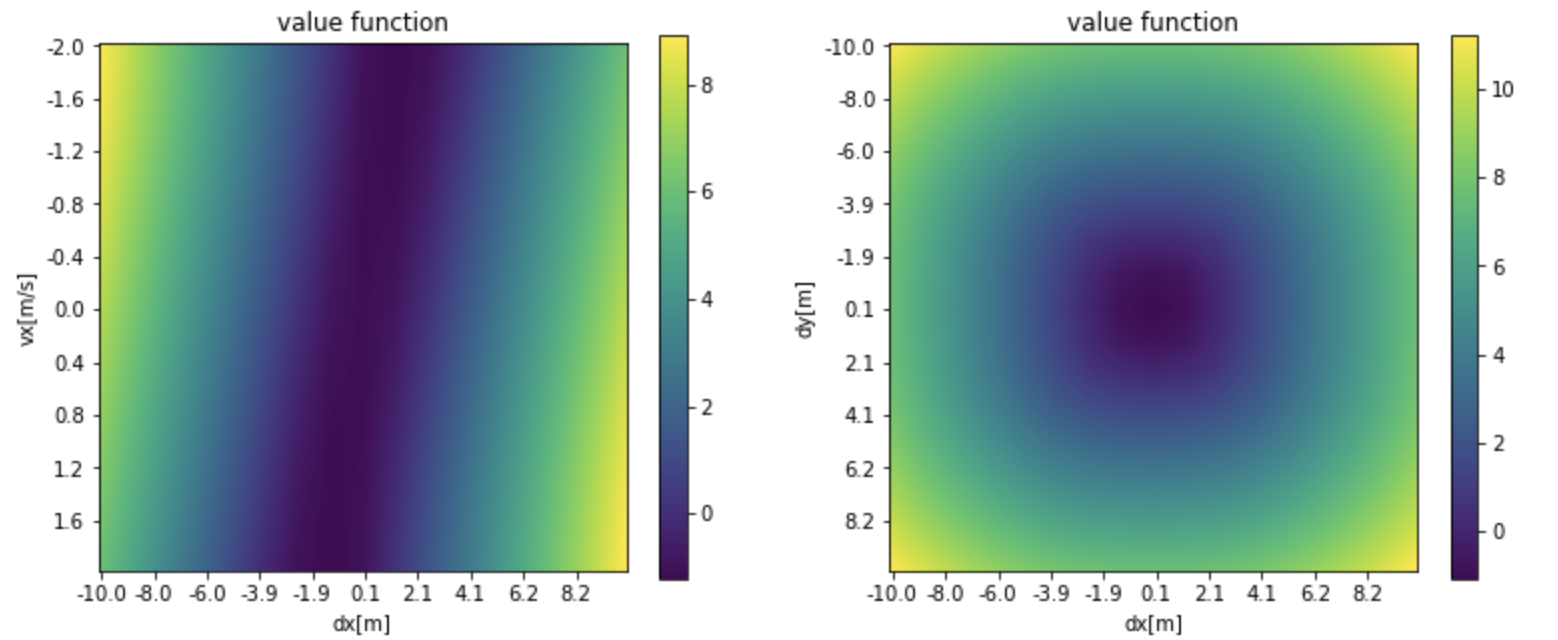
\includegraphics[width=\imgwidth]{images/hj_value_function.png}
\caption{2D slices of 4D \ac{HJR} value function: Position and velocity for one-dimensional case ($y = v_y = 0$, left) and two-dimensional static case ($v_x = v_y = 0$, right)}
\label{img:hj_value_function}
\end{center}
\end{figure}

\subsubsection{Value Function approximation}
Due to the curse of dimensionality the value function cannot be determined with a resolution smaller than $0.5 m$ or $0.5 m/s$, with a feasible amount of pre-computation as well as size of the buffered value function grid and its gradients  on the RAM online \cite{Pavone2020}. There have been several methods for  approximating the value function in post-computation, such as \cite{Zhong2013} comparing the approximate performance of several regression classes such as nearest neighbor or locally weighted projection regression (LMDP) or \cite{Kuper2018} about verifiable safety-critical deep networks. It turns out that using nearest neighbor already lowers the control cost and improves stabilization capability of the value function based MPC control system for diverse (simple) experimental setups such as inverted pendulum, which holds even for time horizons $> 1.5s$. These results motivated comparing several interpolation methods for approximating the value function locally.

\begin{figure}[!ht]
\begin{center}
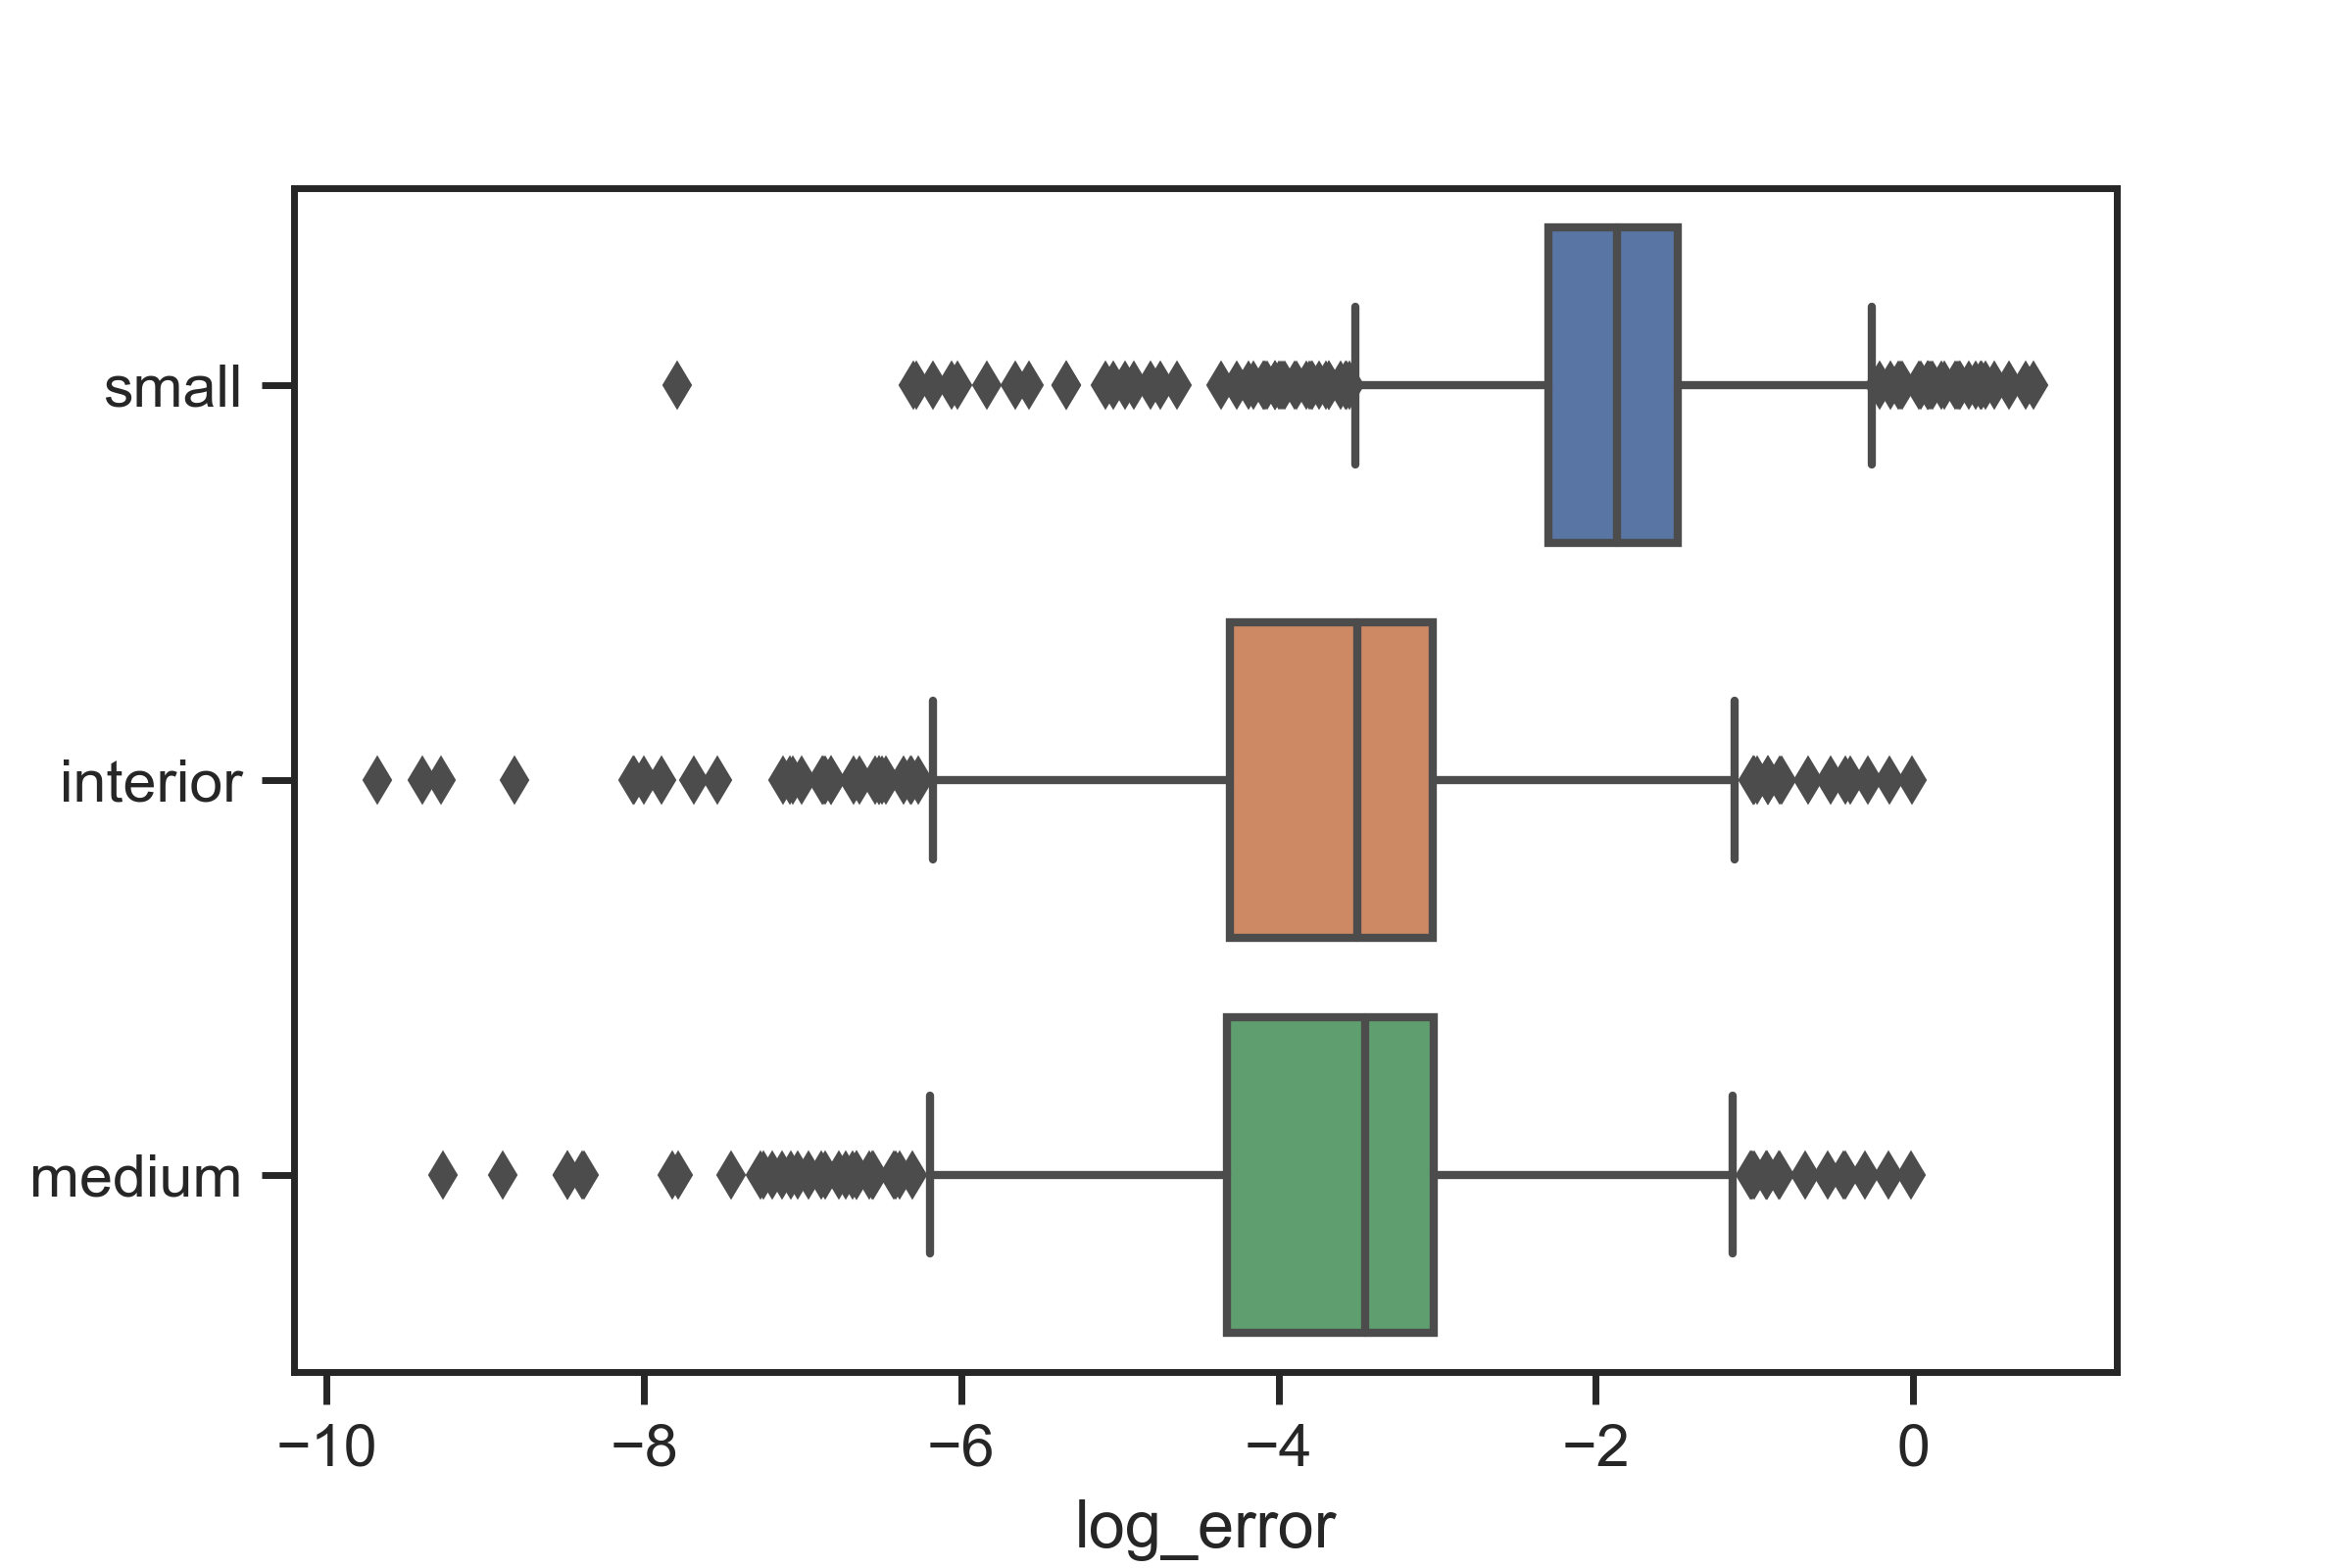
\includegraphics[width=0.45\textwidth]{images/hj_bar_linear.png}
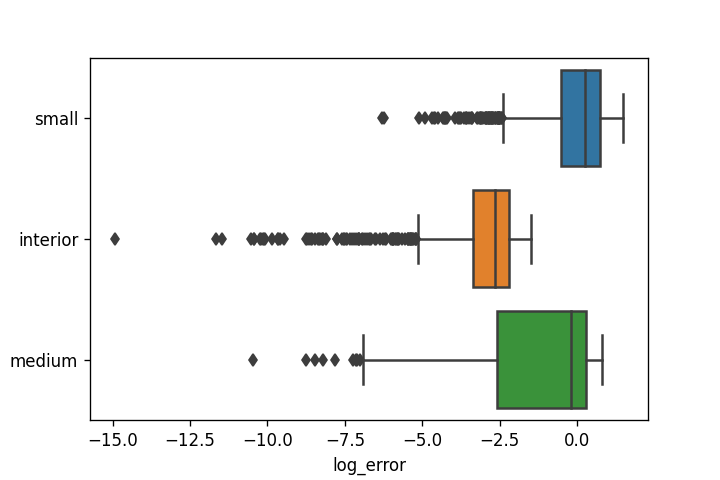
\includegraphics[width=0.45\textwidth]{images/hj_bar_nearest.png}
\caption{Logarithmic value function approximation error using linear (left) and nearest neighbor (right) interpolation methods based on various pre-computed grid sizes (small < interior < medium)}
\label{img:hj_approx_bar}
\end{center}
\end{figure}

\begin{figure}[!ht]
\begin{center}
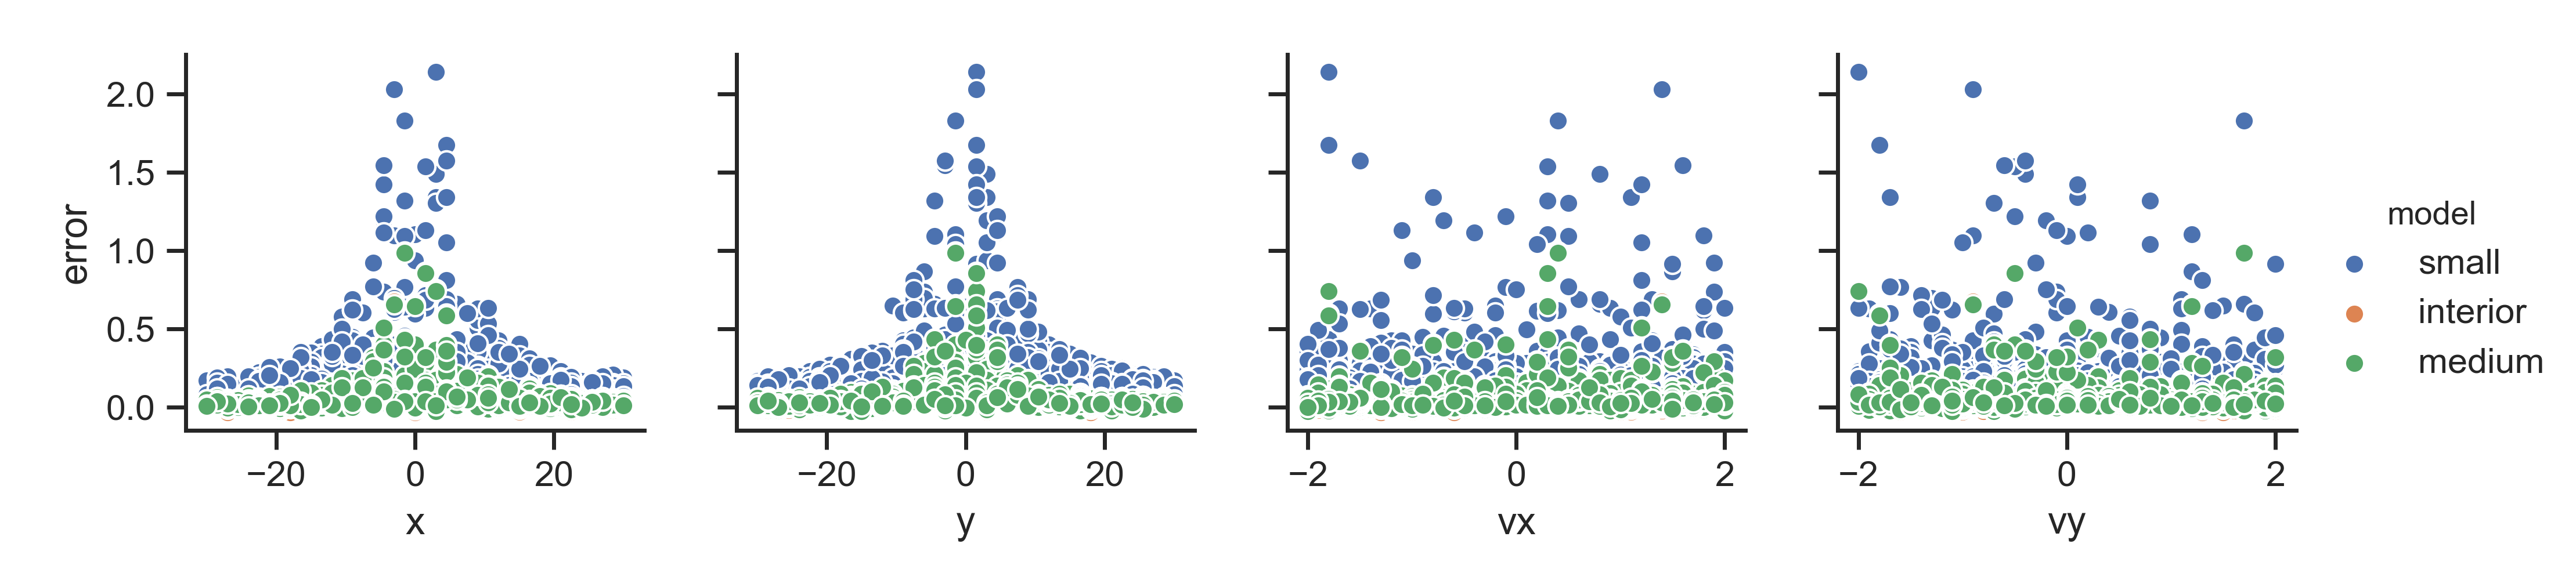
\includegraphics[width=\imgwidth]{images/hj_hist_linear.png}
\caption{Absolute error distribution over joint system state axes using linear interpolation based on various pre-computed grid sizes (small < interior < medium)}
\label{img:hj_approx_hist}
\end{center}
\end{figure}

Figure \ref{img:hj_approx_bar} shows the logarithmic approximation error for several pre-computed grid sizes and using linear (as in \cite{Leung2020}) and nearest neighbor interpolation methods. LWPR (not shown here) has been tested as well but turned out to be infeasible for a large amount of grid points.\footnote{For more information about the implementation of the LWPR value function approximation see \href{https://github.com/simon-schaefer/HJReachibility}{HJ-Reachability Toolbox} on GitHub.} For computing the error metric the value function has been computed on a dense grid exactly, and point-wise compared with the grid interpolated approximations. While linear interpolation widely outperforms nearest neighbor, as expected, the absolute error is very small. As displayed in Figure \ref{img:hj_approx_hist} the interpolation error is not uniform over all joint state axes, but larger for positional axes (which likely is due to the larger amount of non-linearity in position compared to velocity directions, compare Figure \ref{img:hj_value_function}). Therefore, the number of grid points have not been equally distributed over the axes, but biased to the positional axes (interior), while keeping the overall size of the grid constant. 

\subsubsection{\ac{HJR} safety constraint} 
\cite{Leung2020} presents a safety-constraint, based on the resulting value function's gradient, by defining the set of safety-preserving robot control actions as:

\begin{equation}
\uset_{HJR} (\x_{rel}) = \{ \u: \min_{\boldsymbol{d}} \nabla V (\x_{rel})^T \frel(\x, \boldsymbol{d}) \geq 0 \, | \, \u \in \uset \}
\end{equation}

Since the value function $V$ and its gradient $\nabla V$ are computed offline, the constraint is highly efficient to employ online. As the value function has been computed as backward reachable tube, when starting in a safe set $V > 0$ safety is guaranteed for feasible control actions, over the whole time-horizon $T_{HRJ}$, the value function was computed on. Especially, the constraint only depends on the current state, not on future states. Especially the last property make an \ac{HJR}-based constraint very well-suited for project \project. As previously stated evaluating as well as in particular backward passing through the prediction model is the optimization's computational bottleneck. An \ac{HJR}-based safety constraint as described above is however independent from the prediction model. 
\newline
In opposite to \cite{Leung2020} the value function for the joint robot-pedestrian system is negative almost everywhere (comp. Equation \ref{eq:hj_value_negative}), so that a safety-preserving constraint would be infeasible not matter which action is chosen. Therefore the value function itself is bounded, not pre-serving safety but guarantee to stay safe ($\Vrel \leq 0$).

\begin{equation}
\uset_{HJR} (\xrel) = \{ \u: \min_{\dxped[]} \Vrel(\x_{rel} + \frel(\x, \xped[], \u, \dxped[]) \geq \epsilon  \, | \, \u \in \uset \}
\label{eq:hj_constraint}
\end{equation}

To compute \ref{eq:hj_constraint} the value function for all possible pedestrian actions $\dxped[k]$ is determined, conditioned on the current relative state and the chosen robot's control action $\u$. The minimal value with respect to $\dxped[k]$, which reflects the value function in case of the worst-case scenario, given the robot's action, is constrained to be greater or equal zero. If $\u$ in $\uset_{HJR}$ then the robot is guaranteed to be safe from getting close to the pedestrian $k$ within the \ac{HJR}-time-horizon $T_{HJR} = 1s$. Additionally, the buffer $\epsilon > 0$ takes account for interpolation errors. 
\newline
In general it might occur that the relative state itself is infeasible, i.e. has a value term smaller than zero. Due to the inequality \ref{eq:hj_value_negative} there is no control action, that can be chosen by the robot, to reach a positive value. To avoid problem infeasibility, the constraint is appended by a slack variable $\eta \leq 0$, which is strongly weighted in the objective function. 

\begin{equation}
\uset_{HJR} (\xrel) = \{ \u: \min_{\dxped[]} \Vrel(\x_{rel} + \frel(\x, \xped[], \u, \dxped[]) + \eta \geq \epsilon  \, | \, \u \in \uset \}
\end{equation}

\subsubsection{\ac{HJR} multi-agent coupling}
In reality, 

\begin{figure}[!ht]
\begin{center}
\begin{tikzpicture}

    \node[inner sep=0pt] (ped1) at (5,1)
    {
\includegraphics[width=.03\textwidth]{images/walking.png}};
    \fill[orange, opacity=0.3] (ped1) circle (1);
    \draw[dashed, ->] (ped1) to (4, 0);
    
    \node[inner sep=0pt] (ped2) at (-3,-1)
    {
\includegraphics[width=.03\textwidth]{images/walking.png}};
    \fill[orange, opacity=0.3] (ped2) circle (1);
    \draw[dashed, ->] (ped2) to (-1, 0);
    
    \node[inner sep=0pt] (ped3) at (0,2)
    {
\includegraphics[width=.03\textwidth]{images/walking.png}};
    \fill[orange, opacity=0.3] (ped3) circle (1);
    \draw[dashed, ->] (ped3) to (-1, 1);
    
    \node[inner sep=0pt] (ped4) at (2,-1)
    {
\includegraphics[width=.03\textwidth]{images/walking.png}};
    \fill[orange, opacity=0.3] (ped4) circle (1);
    \draw[dashed, ->] (ped4) to (1, -1);
    
    \node[inner sep=0pt] (robot) at (-0.5,0)
    {
\includegraphics[width=.04\textwidth]{images/robot.png}};
    
    \draw [thick] (robot) to[out=0, in=180] (5,3) to[out=0, in=180] node[above, sloped] {$\Vrel \geq 0$ ??} (10, 1);  
    
\end{tikzpicture}
\end{center}
\caption{Avoid set for static ($\dxped[]_t = 0$), single pedestrian scenario}
\label{img:hj_game_multiagent}
\end{figure}



%The system dynamics f : Z ×U → Z is assumed to be uniformly continuous, bounded, and Lipschitz continuous in z for fixed u. 
% any finite number of subsystems defined in the analogous way; however, for clarity and without loss of generality, in this paper we will assume that there are two subsystems.
% intuitively (12) means that the evolution of states in each subsystem depend only on the states in that subsystem: for example, the evolution of x1 depends only on the states in x1. However, the two subsystems are coupled through the state partition y3. 
% Although there may be common or overlapping states in x1 and x2, the evolution of each subsystem does not depend on the other explicitly. In fact, if we for example entirely ignore the subsystem x2, the evolution of the subsystem x1 is well-defined and can be considered a full system on its own; hence, each subsystem is self-contained. ==> each pedestrian plays its own catch-run game, independent from the actions of the other agents
% where the full unsafe set is the intersection of the back projections of subsystem unsafe sets.
% We assume that the full system unsafe set L can be written in terms of the subsystem unsafe sets Lx1 ∈ X1,Lx2 ∈ X2 in the way depicted in Fig. 3:
% Specifically, we will show that if the unsafe set can be decomposed in the way described by (21), then the full-dimensional BRS is decomposable in the same way:


\section{Runtime optimization}
\label{text:approach/runtime}
\subsection{Efficient Trajectory Unrolling}
\label{text:approach/runtime/unrolling}
One of the most promising directions for decreasing the runtime of a trajectory optimization algorithm is to decrease the runtime of the objective and constraints evaluation as well as their gradients. As shown in sections \ref{text:approach/objective} and \ref{text:approach/constraint}, the majority of these optimization modules depend on the robot's trajectory $\x_{0:T}$, rather than on its control inputs $\u_{0:T}$. However, since control inputs are optimized, as described in Section \ref{text:approach/overview}, a computationally efficient transformation from controls and initial state to the trajectory is key for making the trajectory optimization real-time feasible.
\newline
Fortunately, we assumed that the robot follows double integrator dynamics, which are linear and markovian. Hence, they can be expressed as the following: 

\begin{equation}
\x_{t+1} = A \x_t + B \u_t
\label{eq:dynamics}
\end{equation}

\begin{minipage}{0.5\textwidth}
$$A = \begin{bmatrix} 1 & 0 & \dt & 0 \\ 0 & 1 & 0 & \dt \\ 0 & 0 & 1 & 0 \\ 0 & 0 & 0 & 1\end{bmatrix}$$
\end{minipage}
\begin{minipage}{0.5\textwidth}
$$B = \begin{bmatrix} 0 & 0 & \dt & 0 \\ 0 & 0 & 0 & \dt \end{bmatrix}$$
\end{minipage}

Due to the linear (not linearized !) dynamics $\dt = \Delta t$ can be safely used. To fully "unroll" a trajectory, the linear dynamic equation \ref{eq:dynamics} would be applied iteratively for the length of the trajectory. Since the dynamics themselves are linear (not just a first-order approximation), this computation can be further batched and, in this way, speed up. In fact, the full trajectory can be derived merely based on the initial state $\x_0$ and the control input matrix $\u_{0:T}$, as shown in the following:

\begin{align}
\x_1 &= A \x_0 + B \ u_0 \\
\x_2 &= A \x_0 + B \ u_1 = A^2 \x_0 + A B \ u_0 + B \ u_1\\
\hdots &= \hdots \\
\begin{bmatrix} \x_1 \\ \x_2 \\ \vdots \\ \x_n \end{bmatrix} &= \underbrace{\begin{bmatrix} A \\ A^2 \\ \vdots \\ A^n \end{bmatrix}}_{\substack{A_n}} \x_0 + \underbrace{\begin{bmatrix} B & 0 & \hdots & \hdots & 0 \\ AB & B & 0 & \hdots & 0 \\ \hdots & \hdots & \hdots & \hdots & \hdots \\ A^{n-1} B & A^{n-2} B & \hdots & \hdots & B \end{bmatrix}}_{\substack{B_n}} \begin{bmatrix} \u_0 \\ \u_1 \\ \vdots \\ \u_{n-1} \end{bmatrix}
\end{align}

In summary, we get the following (also linear) expression for computing the full robot trajectory at once. As demonstrated in \href{https://github.com/simon-schaefer/mantrap/blob/master/examples/timing.ipynb}{examples/tools/timing} using the fully batched formulation speeds up the trajectory "unrolling" by about a factor of 30.

\begin{equation}
\x_{1:n} = A_n \x_0 + B_n \u_{0:T-1}
\label{eq:dynamics_stacked}
\end{equation}

\subsection{Warm Starting}
\label{text:approach/runtime/warm_starting}
It is widely known that warm starting an optimization can be very beneficial for its convergence speed for several optimization algorithms, e.g. shown in \cite{Banerjee2020} for \ac{GuSTO} or for \ac{IPOPT} in \cite{Shahzad2010}, \cite{John2008} or \cite{Spielberge2019}.
\newline
Within project \project the algorithm has been warm-started by solving the optimization problem posed in problem \ref{eq:formulation} while ignoring all objectives and constraints that relate to pedestrians, i.e. by solving the following optimization problem: \\

\begin{problem}{Simplified optimization problem for warm-starting}
\begin{align}
\min_{\u_{0:T-1}} \quad & J_{goal}(\x_{0:T}) \\
\textrm{s.t. } \quad & \x_{t+1} = \f(\x_t, \u_t) & \forall t \in [0, T - 1] \\
& \x \in \xset & \forall t \in [0, T]\\
& \u_t \in \uset & \forall t \in [0, T]\\
& \x_0 \in \xset_0
\end{align} 
\label{eq:formulation_warm_starting}
\end{problem}

Since the simplified optimization problem in problem \ref{eq:formulation_warm_starting} does not depend on the pedestrian dynamics model $\tilde{\Phi}$ it is much easier and more efficient to solve, being a convex quadratic program. \\

\begin{figure}[!ht]
\begin{center}
\begin{tikzpicture}

    \node (R) at (0, 0) [circle, shade, draw] {Robot};
    \node (G) at (8, 4) [circle, shade, draw] {Goal};
    \node (P1) at (2, 3) [circle, fill=orange, draw] {$P_1$};
    \node (P2) at (8, 1) [circle, fill=yellow, draw] {$P_2$};
    
    \tkzDefPointBy[projection=onto R--G](P1)  \tkzGetPoint{P1m}
    \tkzDefPointBy[projection=onto R--G](P2)  \tkzGetPoint{P2m}
    
    \draw[->, dotted, very thick] (R) to node[above] {} (G);
    \draw (P1m) -- (P1) node[midway, sloped, above] {$\mu_{P1}$};
    \draw (R) -- (P1m) node[midway, sloped, above] {$\eta_{P1}$};
    \draw (P2m) -- (P2) node[midway, sloped, above] {$\mu_{P2}$};
    \draw (R) -- (P2m) node[midway, sloped, below] {$\eta_{P1}$};
    
\end{tikzpicture}
\end{center}
\label{img:robot_goal_encoding}
\end{figure}

%Does the pre-computed set contain every possible scenario? No, but just warm-start so not required, there will be a constrained optimization afterward anyway

\subsection{Attention}
\label{text:approach/runtime/filtering}
For a trajectory optimization to be feasible for online applications, it must be efficient to solve. As empirically shown by experiments in Section \ref{text:experiments/unit}, the computational bottleneck of solving Problem \ref{problem:general} is evaluating and, particularly, differentiating the components, which depend on the interaction between robot and pedestrians. By design, the computational cost of the safety constraint has already been reduced. However, the interactive cost presented in Section \ref{text:approach/objective/interactive} cannot be further runtime optimized or occluded, being one of the core parts of the underlying algorithm. Therefore there are mostly two ways to increase overall runtime efficiency of the trajectory optimization: Firstly, reducing the number of solver iterations for convergence and secondly lowering the runtime cost of evaluating the optimization components itself.
\newline
While the number of solver iterations has already largely been reduced by warm-starting the optimization, the attention focusses on merely taking into account essential factors into the evaluation, with improves runtime without having a significant impact on the resulting behavior of the algorithm. Accurately, the attention filter decides which pedestrians are taken into account for a specific (interactive objective) function evaluation. Importantly to note here, that attention merely effects the evaluation of the interactive objective function (including its gradient computation). Especially, it is not applied to the safety-relevant constraints, to guarantee safety regarding all pedestrians at every time.    
\newline
Using the distance between the robot as each pedestrian is a natural choice for filtering out the agents to consider for the trajectory optimization; the larger the distance is, the smaller the impact of the robot probably is. In fact, the Trajectron model uses a similar distance-based metric for building and evaluating edges in their graph network \cite{Salzmann2020}.

\begin{equation}
\attention(\x, \xped[k]) = \left( ||\x - \xped[k]||_2 > D_{Attention} \right)
\end{equation}

Although euclidean distance-based filtering is a quite naive way of distributing attention to pedestrians in the scene, it shows to be quite effective in reducing the runtime of the interactive objective and gradient evaluations, and therefore of the whole algorithm. A comparison to more sophisticated approaches such as using (forward) reachability to conservatively estimate the pedestrians that eventually could impinge on the robot trajectory, or focussing on only a specific pedestrian instead of a set of pedestrians, as used by game-theoretic crowd navigation works (as presented in Chapter \ref{text:related/crowd_navigation}, e.g.\,  \cite{Bouzat2014}\cite{Nikolaidis2017}), is given in Section \ref{text:experiments/unit}.

